\documentclass[11pt, a4paper]{article}
%\usepackage{proj1}
\usepackage{natbib}
\usepackage{fancyhdr}  
\usepackage{subcaption}
\usepackage{caption}
\usepackage{graphicx}
\linespread{1.25} 
\setlength{\parindent}{0cm}
\graphicspath{{Images/}}
\usepackage{hyperref}
\usepackage{amsmath}
\usepackage{amsfonts}
\usepackage{amssymb}
\usepackage{amsthm}
\usepackage{mathtools}
\usepackage{commath}

%\usepackage[sc,osf]{mathpazo}
\usepackage{subcaption}
\usepackage[a4paper, top=1in, left=1.0in, right=1.0in, bottom=1in, includehead, includefoot]{geometry} %Usually have top as 1in

\usepackage{listings}
\usepackage{color} %red, green, blue, yellow, cyan, magenta, black, white
\definecolor{mygreen}{RGB}{28,172,0} % color values Red, Green, Blue
\definecolor{mylilas}{RGB}{170,55,241}


\hypersetup{colorlinks,linkcolor={black},citecolor={blue},urlcolor={black}}
\usepackage{color}
\urlstyle{same}


\theoremstyle{definition}
\newtheorem{definition}{Definition}[section]

\title{Exact Solutions for the Full Problem \\with Force Control and with Flow Control}
\date{}
\newcommand{\Sta}{\rho}
\newcommand{\Adj}{p}
\newcommand{\Con}{u}

\pagenumbering{gobble}
\begin{document}
\section*{Report 23/04/2020 (Part 3)}
For all problems we choose ODE tols $ = 10^{-8}$, consistency tols $= 10^{-4}$, $n=61$, $N= 60$ and force or flow are zero in the forward problems. We choose FixPt solver throughout. Results still to be verified with Picard.
\section{Force Control - Dirichlet}
The aim is to show a force control problem with particle interactions. Problem: generally the three choices of $\gamma = -1,0,1$ give almost identical results for a range of initial conditions and targets.
$\gamma =2,-2$ and $D_0 = 0.5$ shows some difference in the forward problem.\\
Staying with $\gamma = -1,0,1$ and $D_0 =1$, we get the following results.
With $\gamma = 0$ and $\beta = 10^{-3}$, the algorithm converges. $J_{FW} = 0.0365 $, $J_{Opt} = 0.0032$, see Figure \ref{rhoDF0}.
With $\gamma = -1$ and $\beta = 10^{-3}$, the algorithm converges. $J_{FW} = 0.0365$, $J_{Opt} = 0.0031$, see Figure \ref{rhoDF1}.
With $\gamma = 1$ and $\beta = 10^{-3}$, the algorithm converges. $J_{FW} = 0.0365 $, $J_{Opt} = 0.0033$, see Figure \ref{rhoDF2}.
We can see the lack of difference in pictures and in cost functional values.
\begin{figure}[h]
	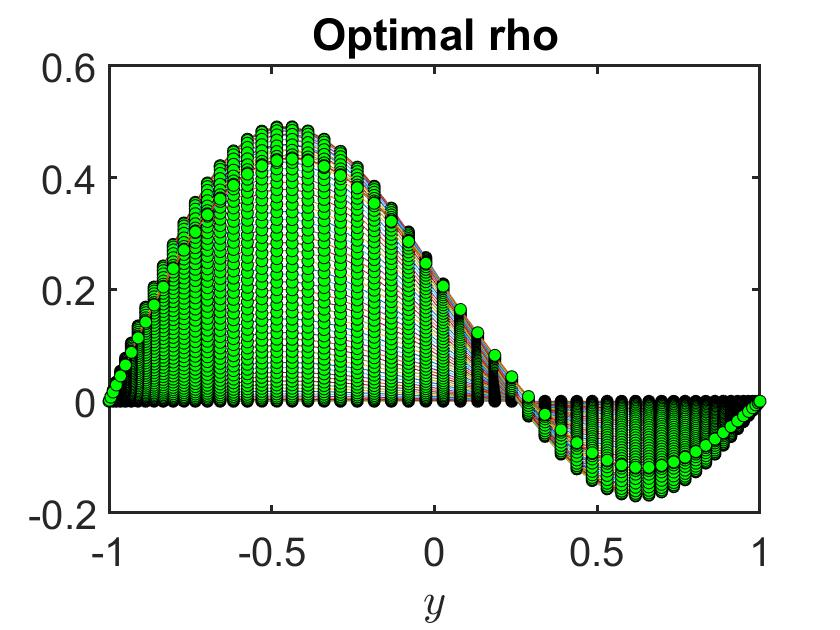
\includegraphics[scale=0.3]{DFrhoOpt0.jpg}
	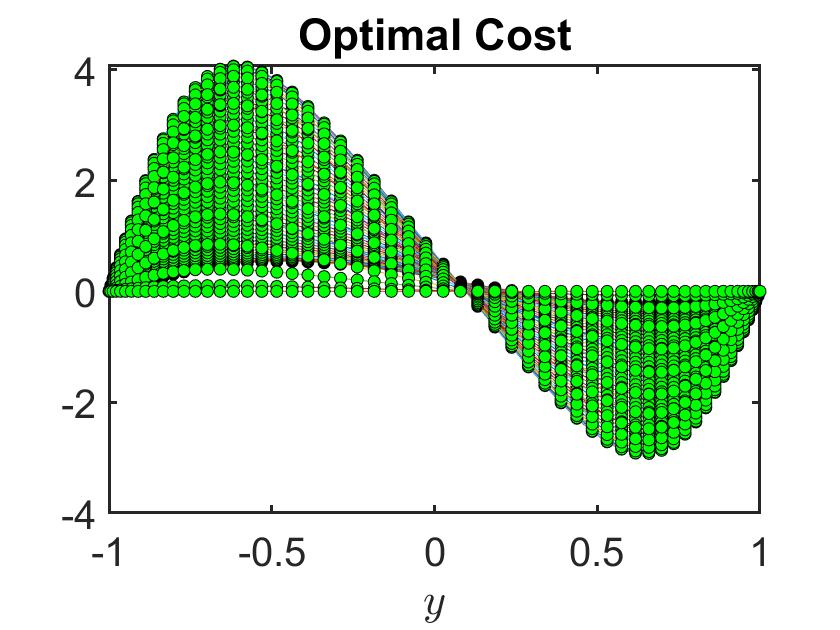
\includegraphics[scale=0.3]{DFwOpt0.jpg}
	\caption{Solution $\rho_{Opt}$ and $w_{Opt}$, with $\gamma = 0$ and $D_0 = 1$.}
	\label{rhoDF0}
\end{figure}

\begin{figure}[h]
	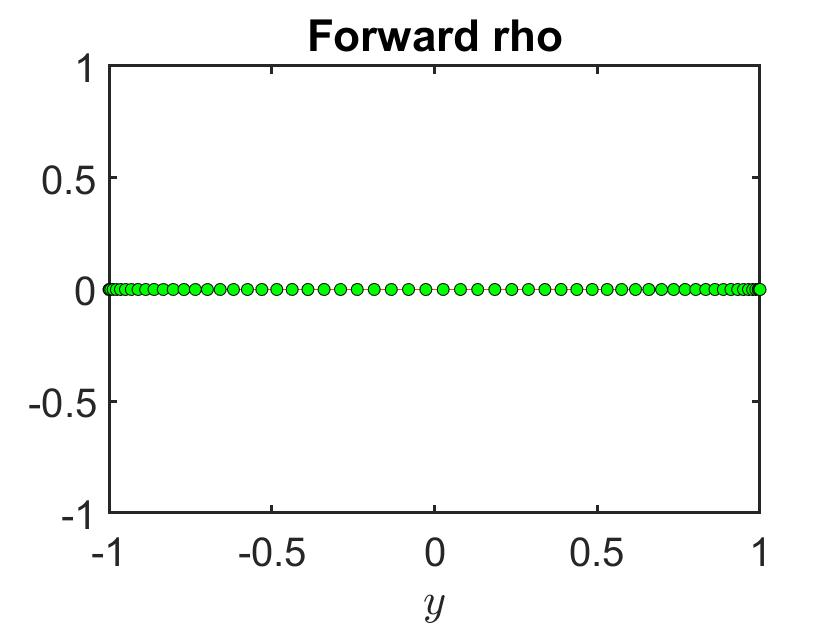
\includegraphics[scale=0.3]{DFrhoFW1.jpg}	
	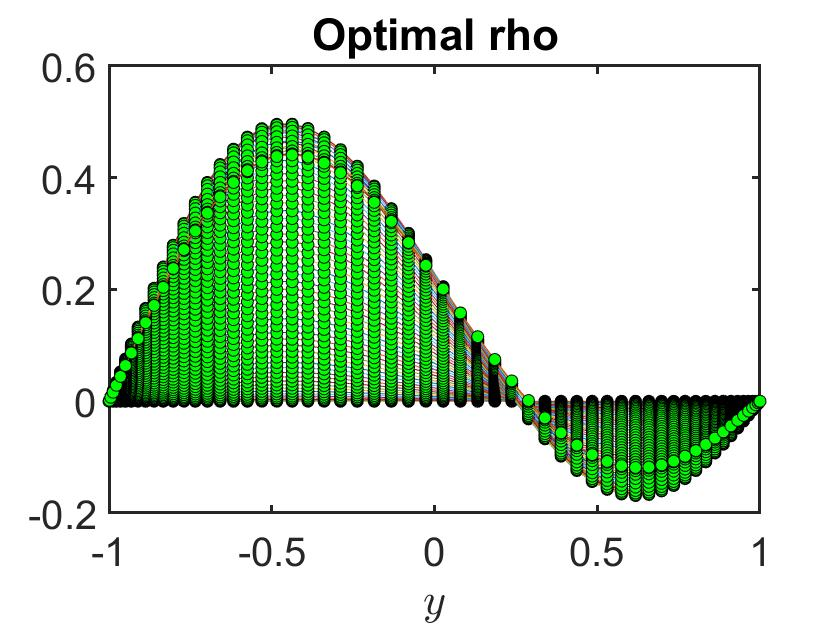
\includegraphics[scale=0.3]{DFrhoOpt1.jpg}
	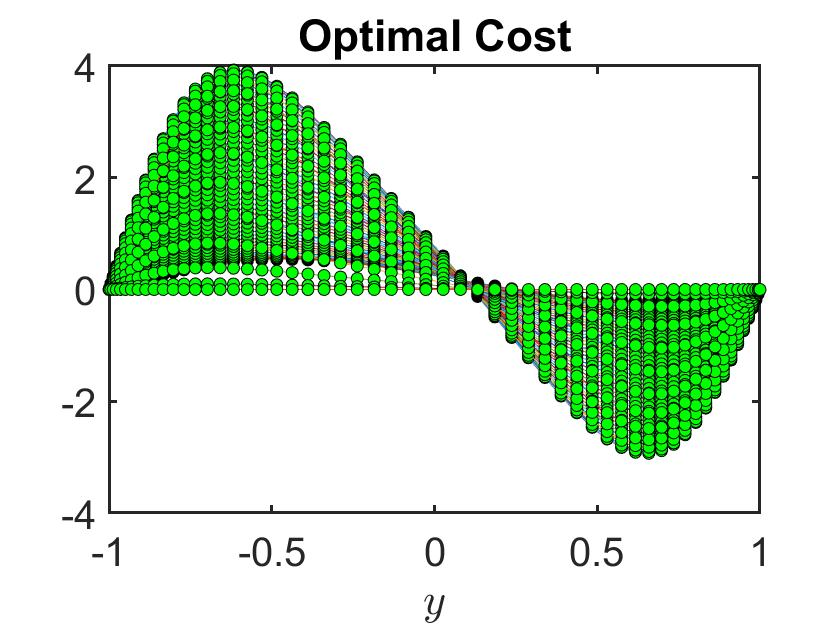
\includegraphics[scale=0.3]{DFwOpt1.jpg}
	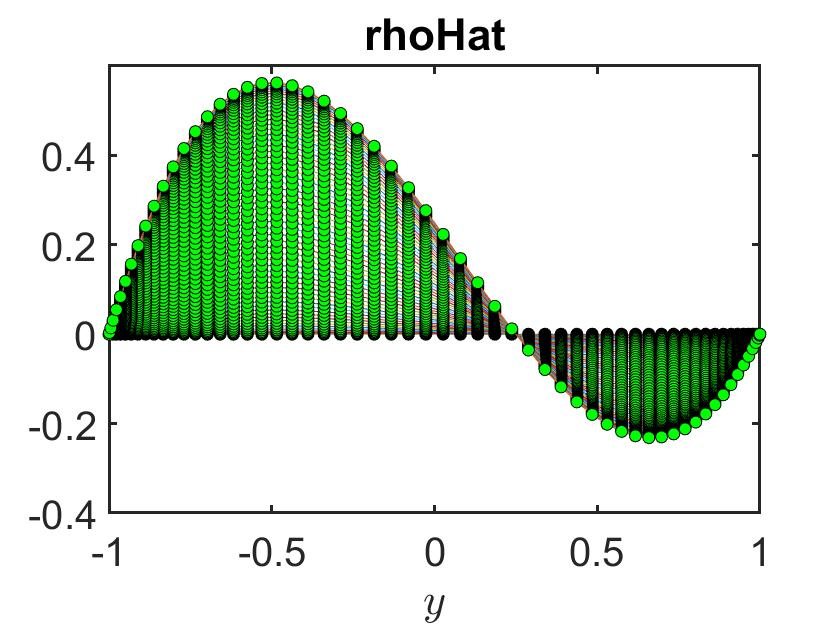
\includegraphics[scale=0.3]{DFrhoHat1.jpg}
	\caption{Solutions $\rho_{FW}$ and $\rho_{Opt}$, $\hat \rho$ and $w_{Opt}$, with $\gamma = -1$ and $D_0 = 1$.}
	\label{rhoDF1}
\end{figure}
\begin{figure}[h]
	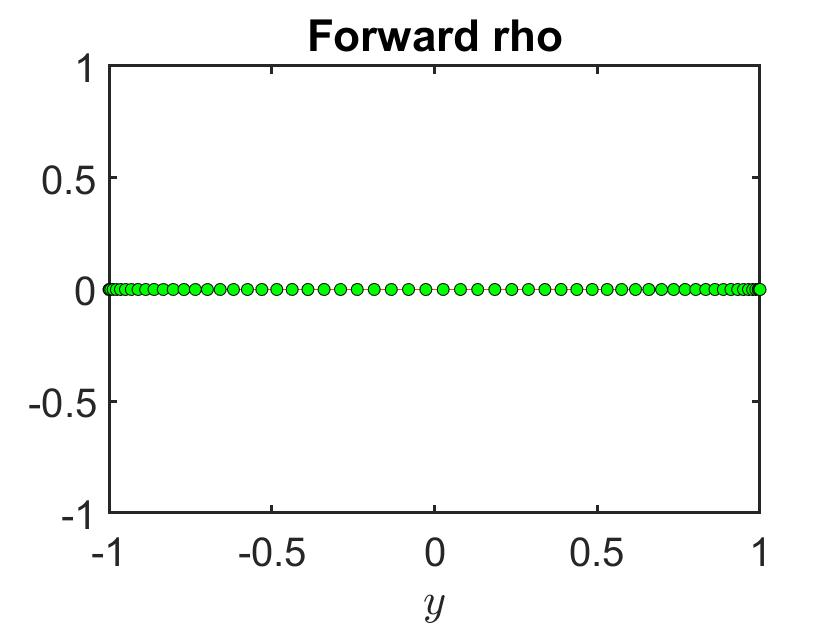
\includegraphics[scale=0.3]{DFrhoFW2.jpg}	
	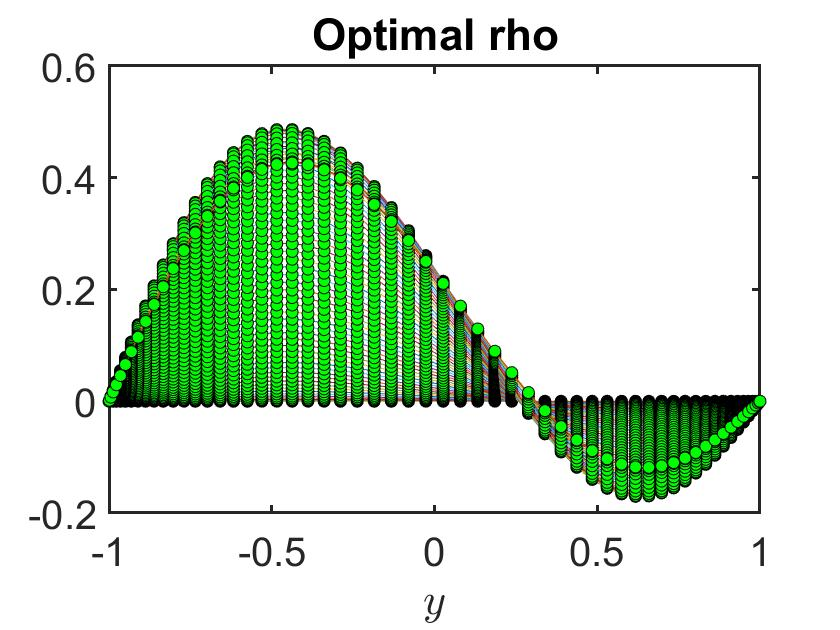
\includegraphics[scale=0.3]{DFrhoOpt2.jpg}
	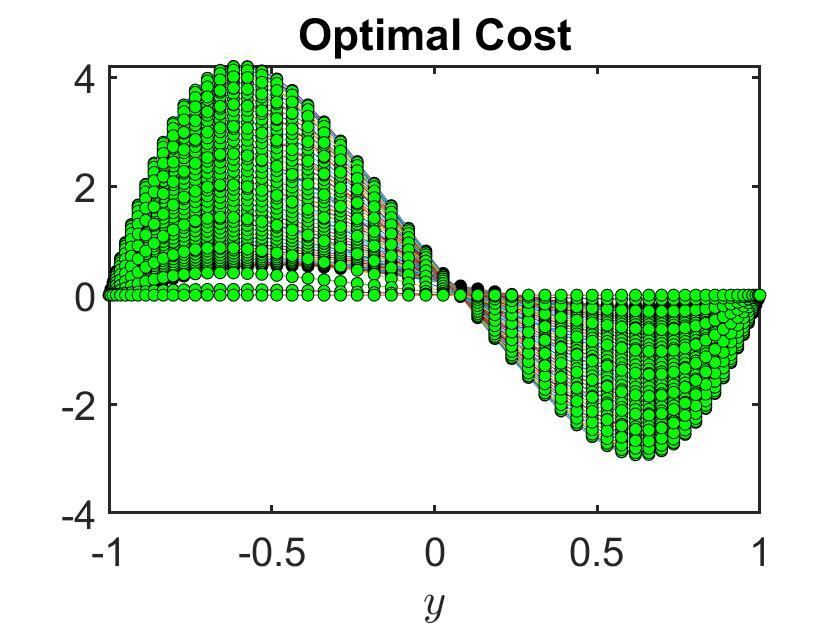
\includegraphics[scale=0.3]{DFwOpt2.jpg}
	\caption{Solutions $\rho_{FW}$ and $\rho_{Opt}$,  and $w_{Opt}$, with $\gamma = 1$ and $D_0 = 1$.}
	\label{rhoDF2}
\end{figure}
\section{Force Control - Neumann}
We choose the same configurations as in the Flow control case (moving target 1):
\begin{align*}
\hat \rho = (1-t)0.5 + t\frac{1}{4}(\cos(\pi y + \pi) + 2),
\end{align*}
and the initial condition for $\rho$ is:
\begin{align*}
\rho_{IC} = 0.5.
\end{align*}
For $\gamma = 0$, $\beta = 10^{-3}$ it converges, but only if $\lambda = 0.001$. Then $J_{FW} = 0.0104$, $J_{Opt}= 0.0011$, see Figure \ref{rhoNF0}.\\
Try $\gamma = -1$. This converges in $6506$ iterations (similar to $\gamma =0$ $25$ min). $J_{FW} = 0.0041$, $J_{Opt} = 4.7534 \times 10^{-4}$, see Figure \ref{rhoNF1}. Comparing the two figures, there is not much difference in the solutions of $\gamma =0$ and $\gamma = -1$, however, the values of the cost functionals are very different, since for $\gamma =-1$ the forward solution is already closer to $\hat\rho $, while the forward solution for $\gamma =0$ is constant.\\
Choosing $\gamma = 1$ converges as well in a similar time frame. $J_{FW} = 0.0195$, $J_{Opt} = 0.0023$, see Figure \ref{rhoNF2}. The optimal solution does differ from the previous two, since the repulsive interactions result in a forward solution far from $\hat \rho$.
\begin{figure}[h]
	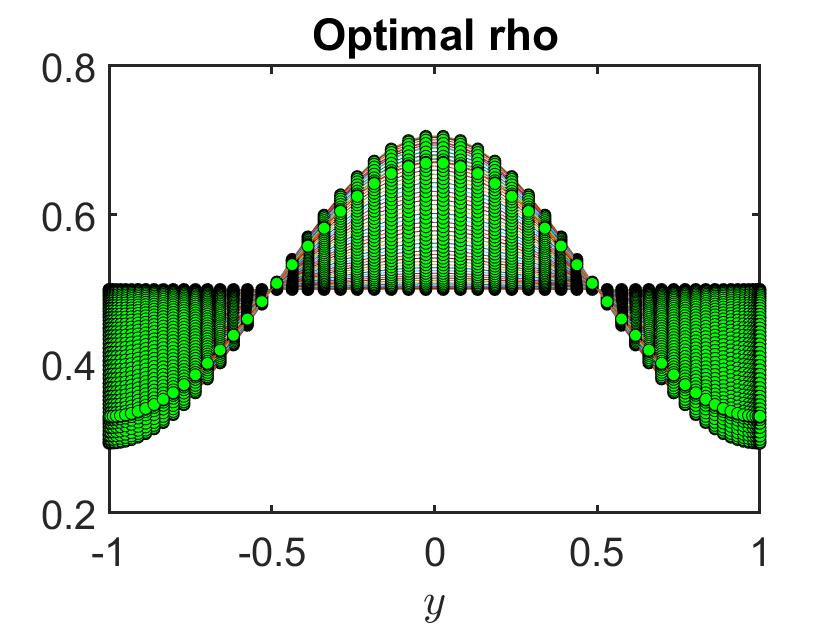
\includegraphics[scale=0.3]{NFrhoOpt0.jpg}
	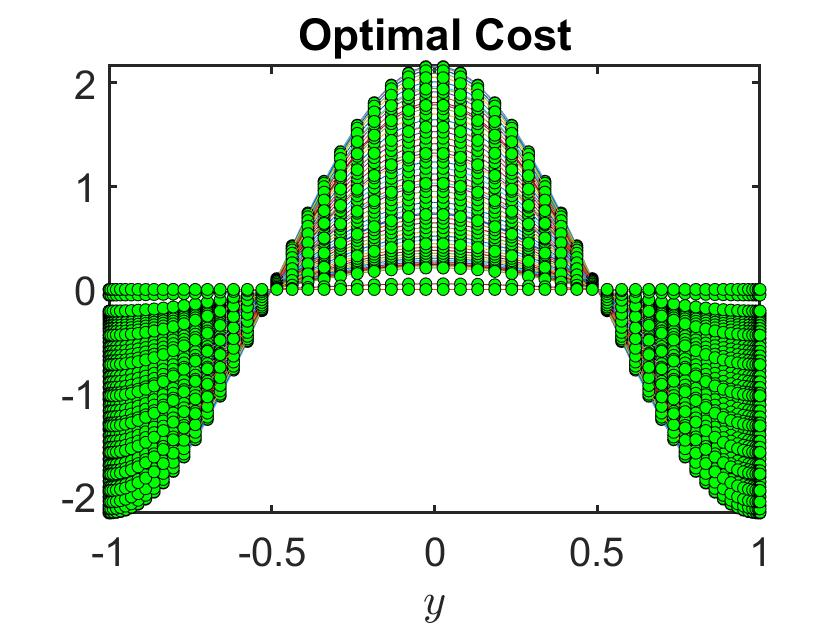
\includegraphics[scale=0.3]{NFwOpt0.jpg}
	\caption{Solution $\rho_{Opt}$ and $w_{Opt}$, with $\gamma = 0$ and $D_0 = 1$.}
	\label{rhoNF0}
\end{figure}
\begin{figure}[h]
	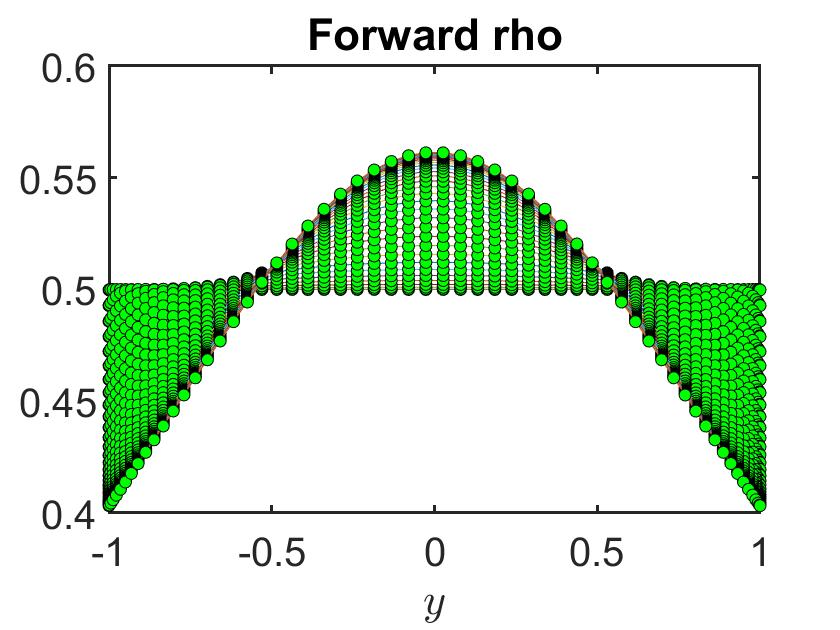
\includegraphics[scale=0.3]{NFrhoFW1.jpg}	
	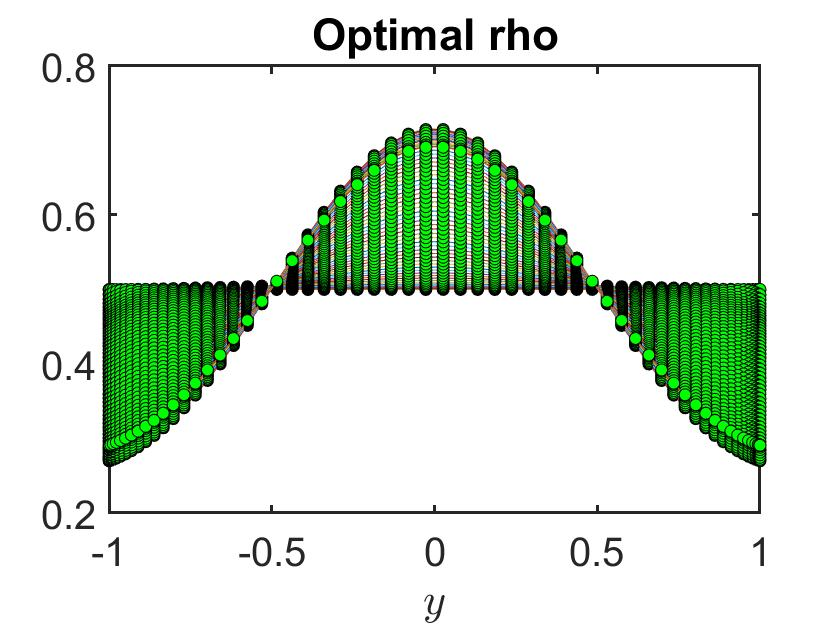
\includegraphics[scale=0.3]{NFrhoOpt1.jpg}
	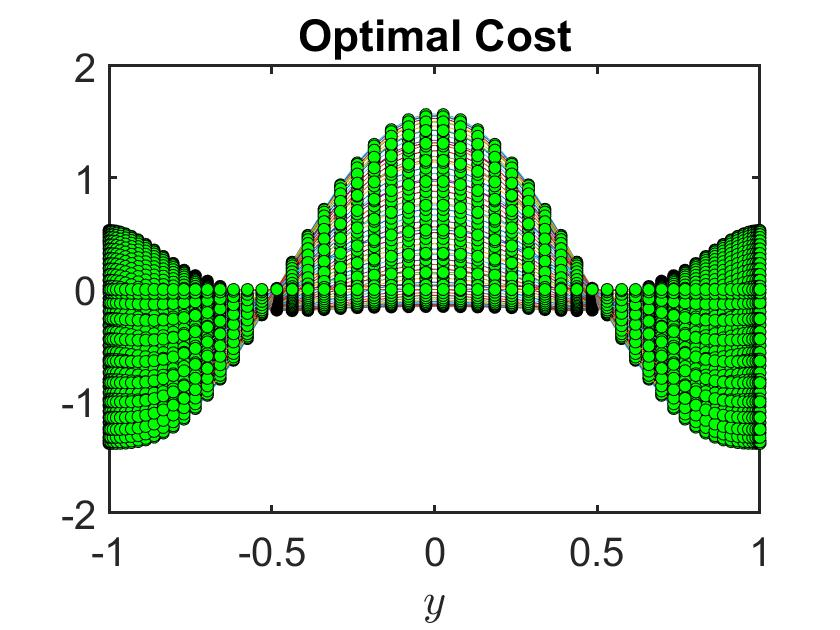
\includegraphics[scale=0.3]{NFwOpt1.jpg}
	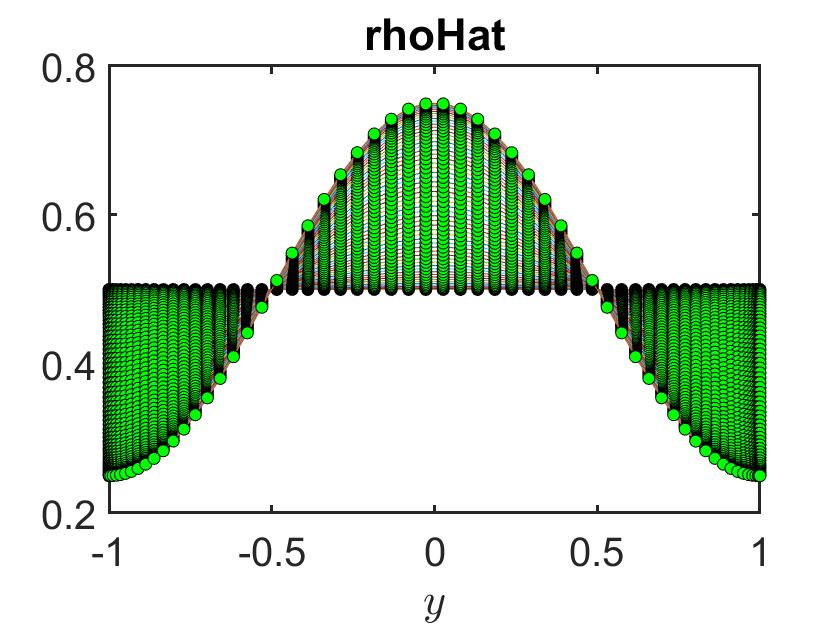
\includegraphics[scale=0.3]{NFrhoHat1.jpg}
	\caption{Solutions $\rho_{FW}$ and $\rho_{Opt}$, $\hat \rho$ and $w_{Opt}$, with $\gamma = -1$ and $D_0 = 1$.}
	\label{rhoNF1}
\end{figure}


\begin{figure}[h]
	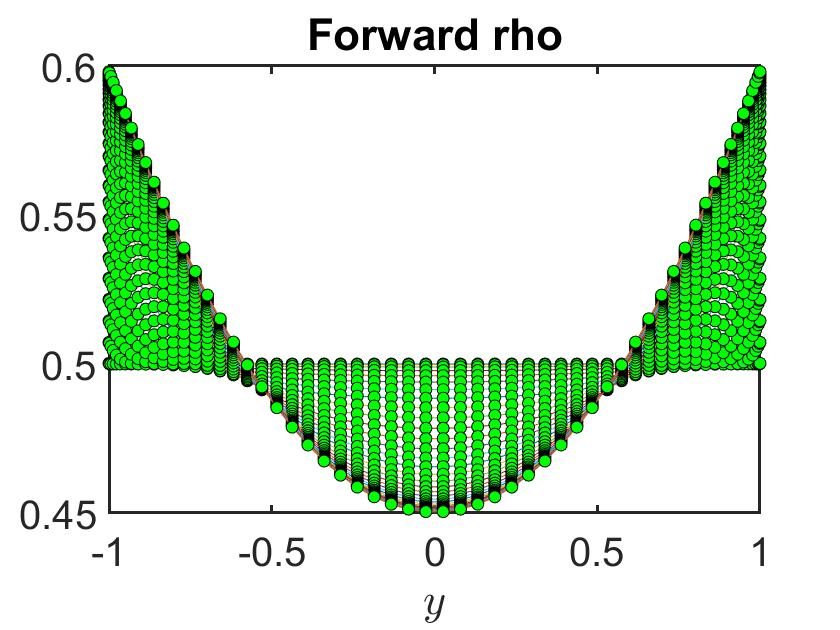
\includegraphics[scale=0.3]{NFrhoFW2.jpg}	
	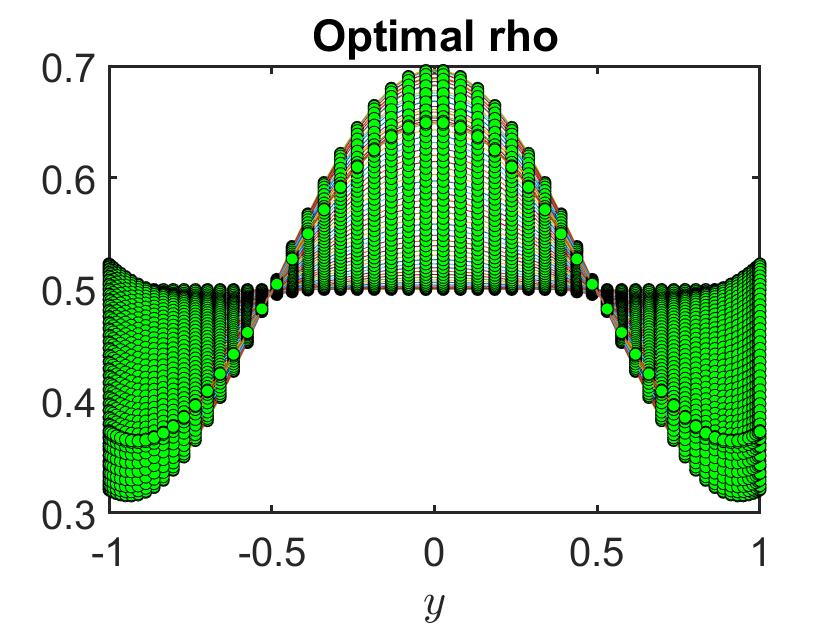
\includegraphics[scale=0.3]{NFrhoOpt2.jpg}
	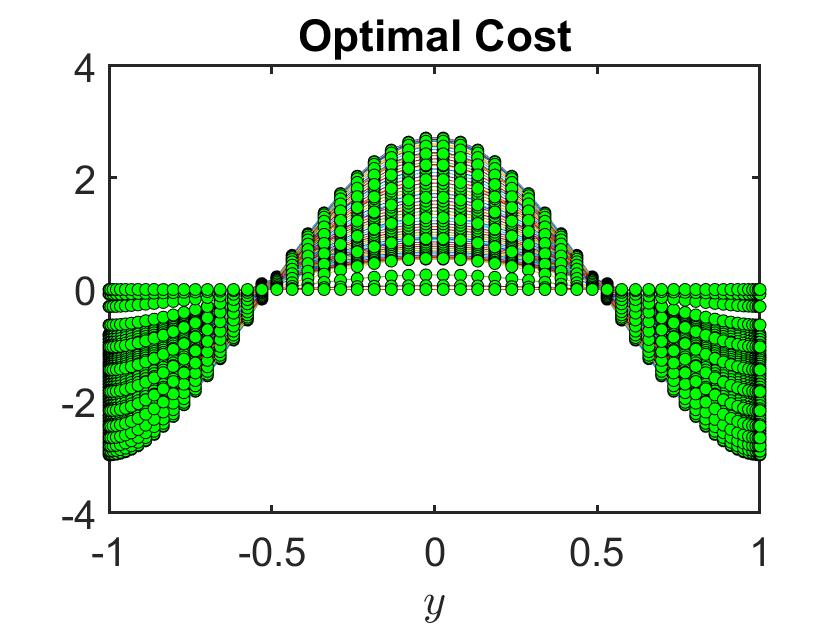
\includegraphics[scale=0.3]{NFwOpt2.jpg}
	\caption{Solutions $\rho_{FW}$ and $\rho_{Opt}$,  and $w_{Opt}$, with $\gamma = 1$ and $D_0 = 1$.}
	\label{rhoNF2}
\end{figure}

\section{Flow Control - Dirichlet}
When using the same approach as in the Neumann case, the solution is a constant zero function (as the only uniform initial condition is the zero function). We therefore need another approach.
The target is a moving target from the initial condition of $\rho$ to a different particle distribution:
\begin{align*}
\hat \rho = (1-t)(-y^3 -(1/4)y^2 + y + 0.25) +  t(y^3 -(1/4)y^2 - y + 0.25).
\end{align*}
The initial condition for $\rho$ is:
\begin{align*}
\rho_{IC}= -y^3 -(1/4)y^2 + y + 0.25.
\end{align*}
At first we try the case $\gamma = 0$, $\beta = 10^{-3}$, $\lambda = 0.01$. This converges in $1013$ iterations ($12$ min, very slow). $J_{FW} = 0.0324$, $J_{Opt} = 0.0180$, see Figure \ref{rhoDFl1}.
\begin{figure}[h]
	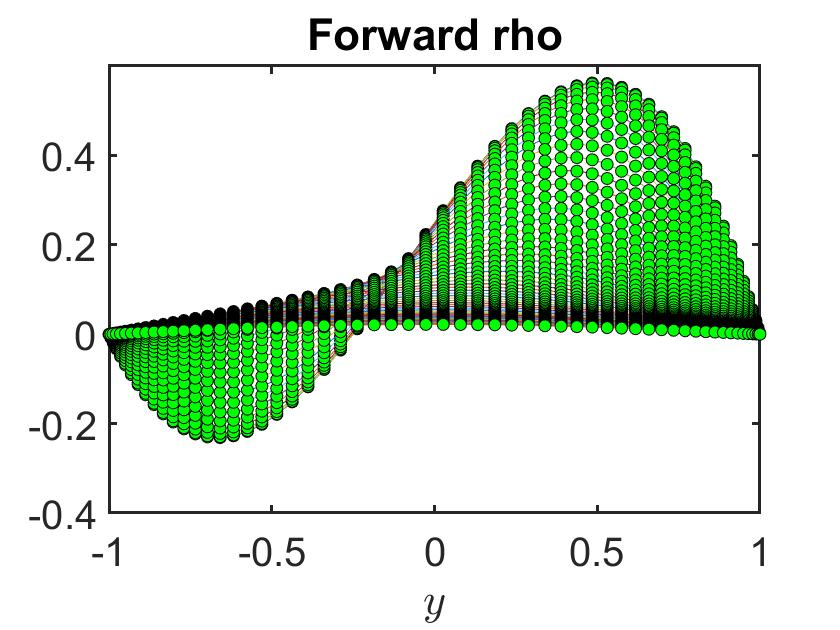
\includegraphics[scale=0.3]{DFlrhoFW1.jpg}	
	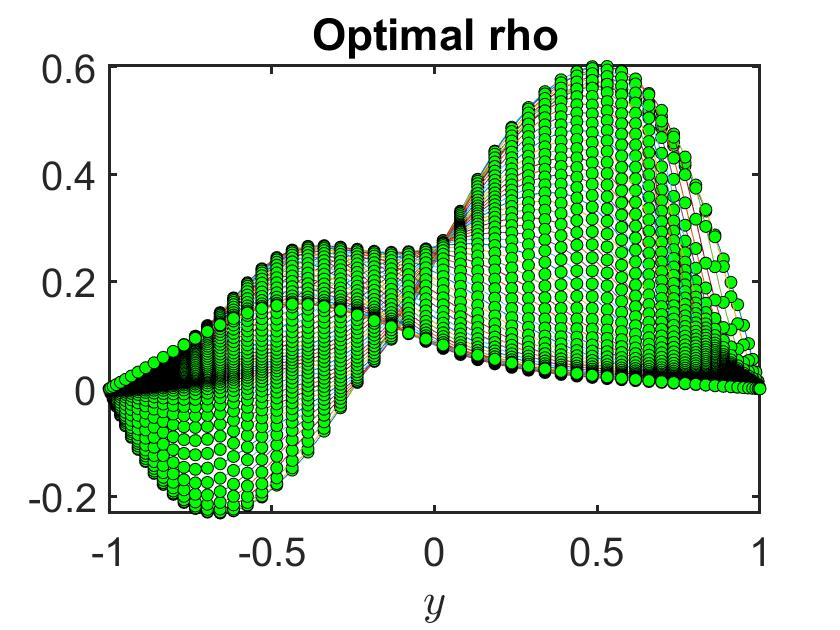
\includegraphics[scale=0.3]{DFlrhoOpt1.jpg}
	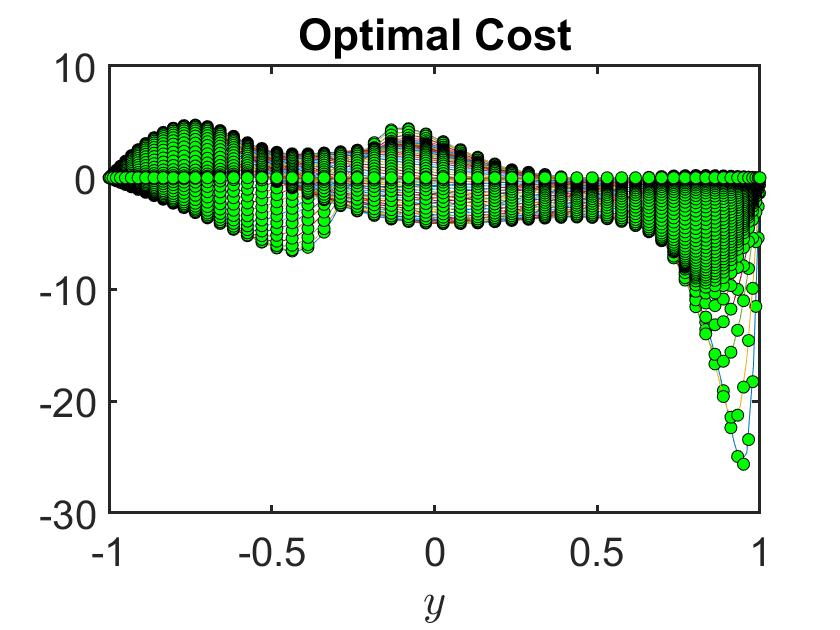
\includegraphics[scale=0.3]{DFlwOpt.jpg}
	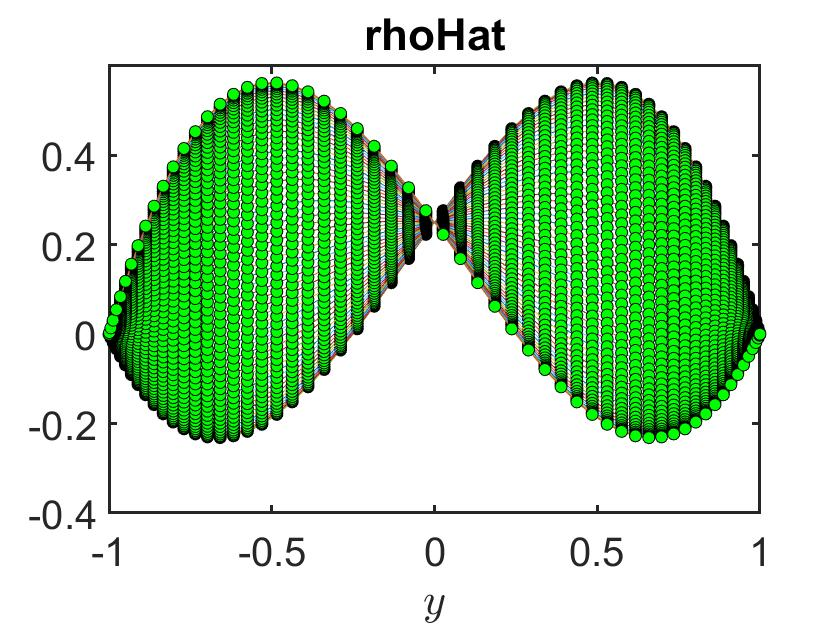
\includegraphics[scale=0.3]{DFlrhoHat1.jpg}
	\caption{Solutions $\rho_{FW}$ and $\rho_{Opt}$, $\hat \rho$ and $w_{Opt}$, with $\gamma = 0$ and $D_0 = 1$.}
	\label{rhoDFl1}
\end{figure}
For $\gamma = -1$ this converges in $1008$ iterations ($11$ min), $J_{FW} = 0.0319$, $J_{Opt} = 0.0175$, see Figure \ref{rhoDFl2}. Overall, these two problems are not very different, so the particle interaction doesn't seem to have a big impact on the results. This needs to be improved.
\begin{figure}[h]
	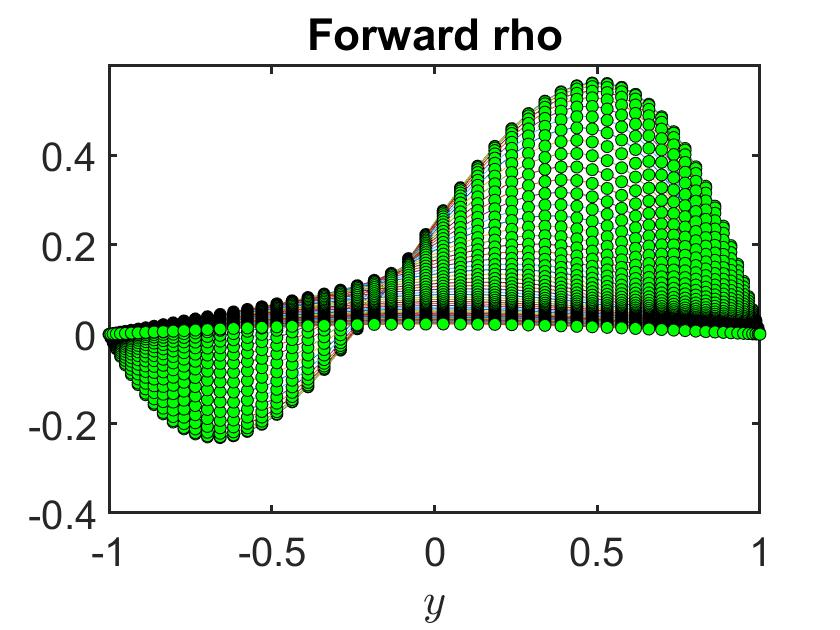
\includegraphics[scale=0.3]{DFlrhoFW2.jpg}	
	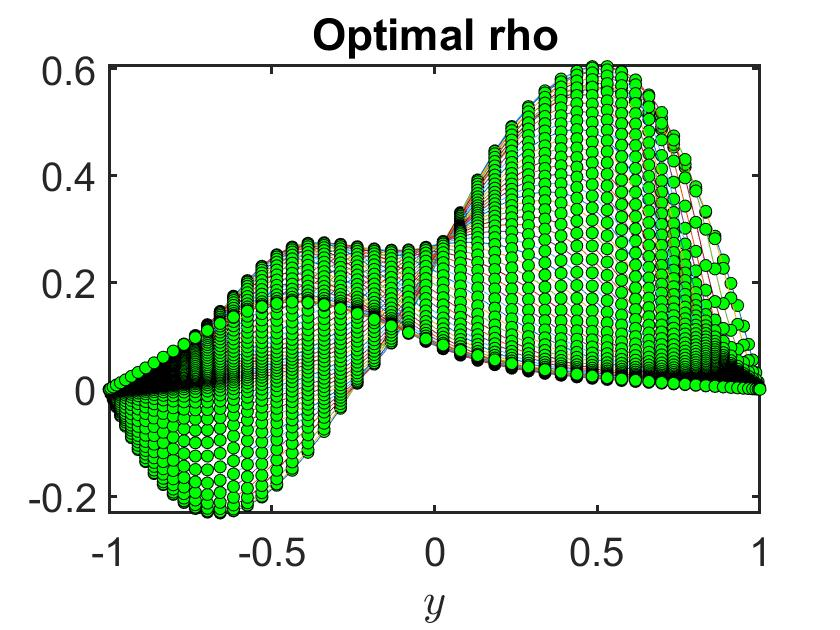
\includegraphics[scale=0.3]{DFlrhoOpt2.jpg}
	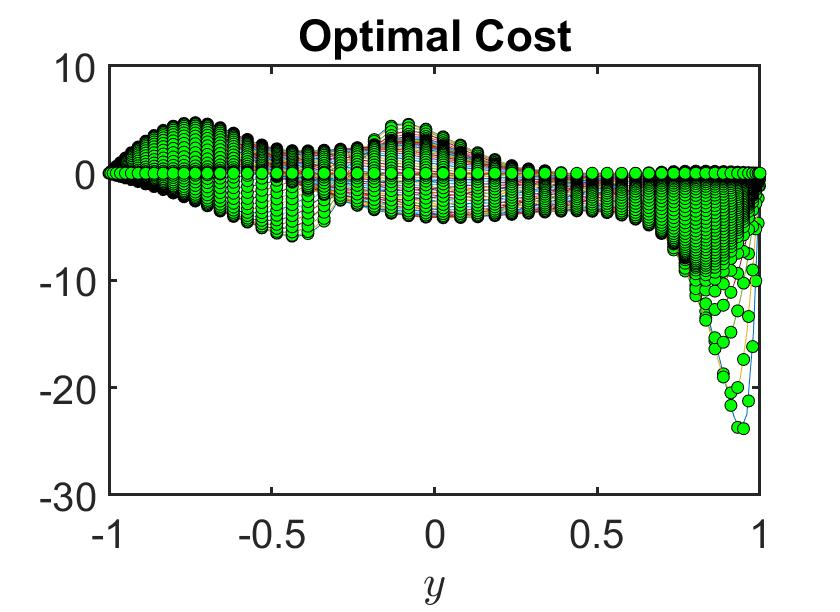
\includegraphics[scale=0.3]{DFlwOpt2.jpg}
	\caption{Solutions $\rho_{FW}$ and $\rho_{Opt}$,  and $w_{Opt}$, with $\gamma = -1$ and $D_0 = 1$.}
	\label{rhoDFl2}
\end{figure}
With $\gamma = 1$, this converges as well, $J_{FW} = 0.0328$, $J_{Opt} = 0.0185$, see Figure \ref{rhoDFl3}. Since the interactions are repulsive, they are slightly acting against $\hat \rho$ direction, so the cost functionals are slightly higher than for the other two values of $\gamma$. However, there is no great difference in the pictures or in the values of the cost functionals.

\begin{figure}[h]
	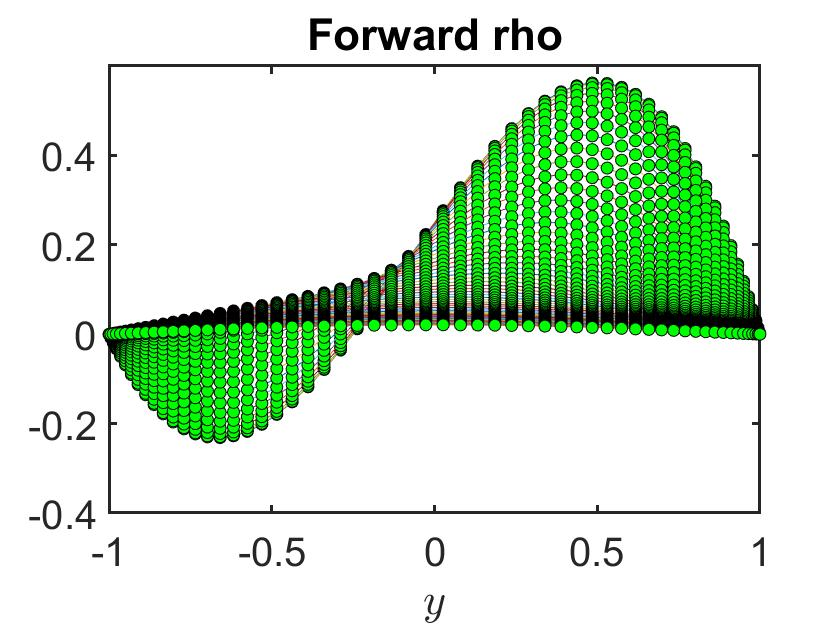
\includegraphics[scale=0.3]{DFlrhoFW3.jpg}	
	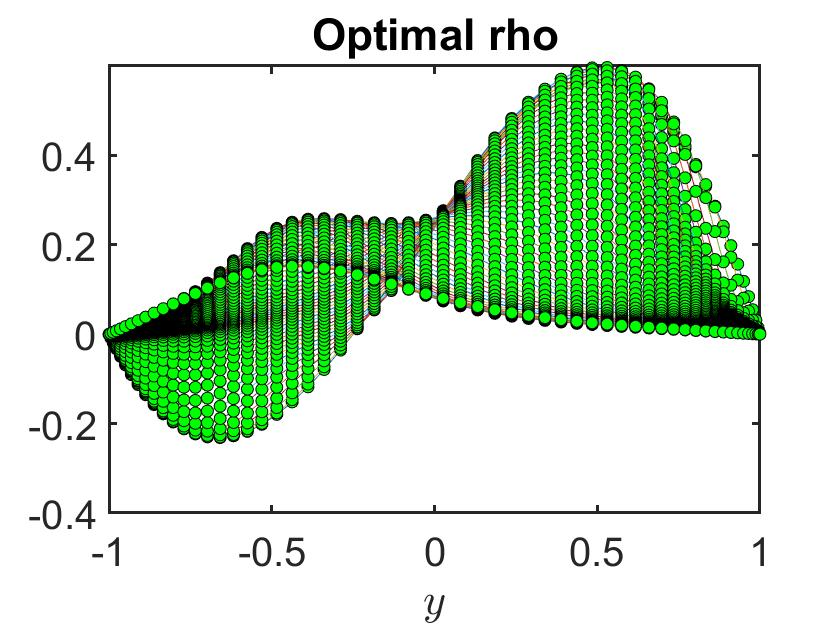
\includegraphics[scale=0.3]{DFlrhoOpt3.jpg}
	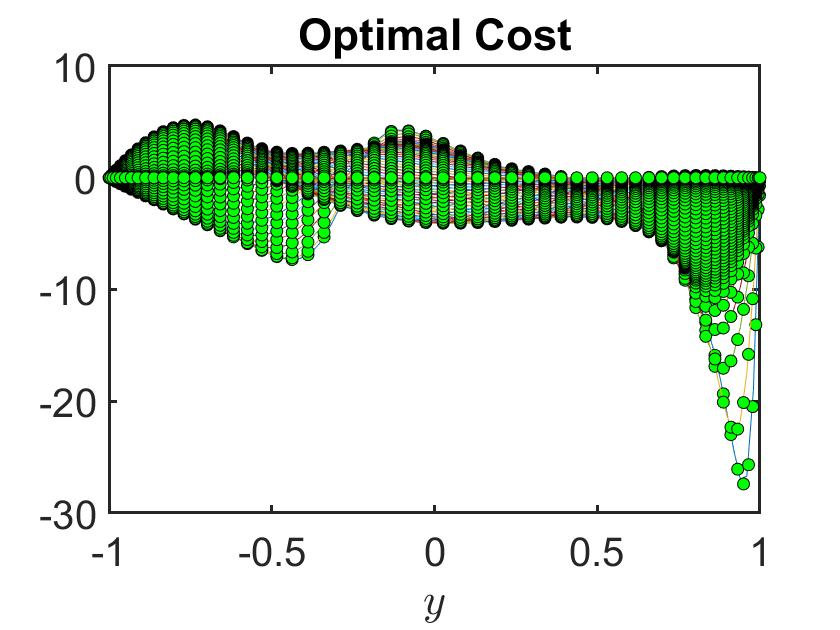
\includegraphics[scale=0.3]{DFlwOpt3.jpg}
	\caption{Solutions $\rho_{FW}$ and $\rho_{Opt}$,  and $w_{Opt}$, with $\gamma = 1$ and $D_0 = 1$.}
	\label{rhoDFl3}
\end{figure}











\end{document}